\documentclass[twoside]{article}
\usepackage[utf8]{inputenc}
\usepackage{amsmath,amsfonts,amssymb,amsthm,latexsym}
\usepackage[spanish,es-noshorthands]{babel}
\usepackage[T1]{fontenc}
\usepackage{lmodern}
\usepackage{graphicx,hyperref}
\usepackage{tikz,pgf}
\usepackage{marvosym}
\usepackage{multicol}
\usepackage{fancyhdr}
\usepackage[papersize={5.5in,8.5in},left=.8cm,right=.8cm,top=1.5cm,bottom=1.3cm]{geometry}
\usepackage{fancyhdr}
\pagestyle{fancy}
\fancyhead[LE]{\Email iedabgerman@autistici.org}
\fancyhead[RE]{}
\fancyhead[RO]{\url{https://www.autistici.org/mathgerman}}
\fancyhead[LO]{}

\author{Germ\'an Avenda\~no Ram\'irez~\thanks{Lic. Mat. U.D., M.Sc. U.N.}}
\title{\begin{minipage}{.2\textwidth}

\includegraphics[height=1.75cm]{Images/logo-colegio.png}\end{minipage}
\begin{minipage}{.55\textwidth}
\begin{center}
Taller 03, ¿Quién dejó esta huella?\\
Geometría $6^{\circ}$
\end{center}
\end{minipage}\hfill
\begin{minipage}{.2\textwidth}
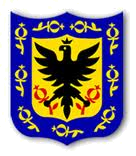
\includegraphics[height=1.75cm]{Images/logo-sed.png} 
\end{minipage}}
\date{}
\thispagestyle{plain}
\begin{document}
\maketitle
 \section*{Lo que s\'e}
 Generalmente, cada vez que nos desplazamos de un lugar a otro, ya sea por nuestros propios medios o utilizando algún tipo de transporte, déjamos huellas fáciles de reconocer y que le permite a los observadores tratar de averiguar de dónde partimos y en qué dirección nos movemos.

En esta guía te invitamos a sacar todos tus dotes de investigador para que nos ayudes a decifrar ¿quién dejó esta huella

\begin{minipage}{.65\textwidth}
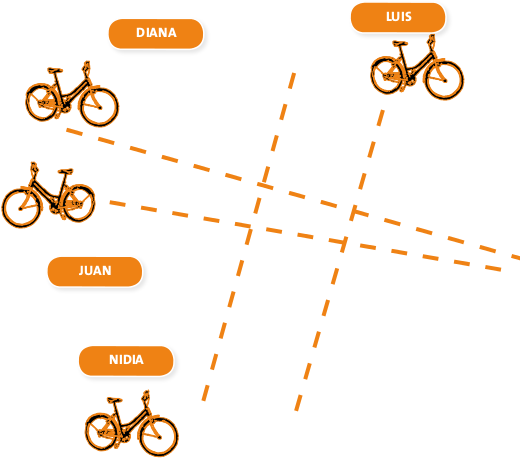
\includegraphics[scale=.45]{Images/Carreras_bicicletas.png}
\end{minipage}\hfill
\begin{minipage}{.3\textwidth}
\begin{itemize}
\item Reúnete con un compañero o compañera. Resuelvan las preguntas.
\end{itemize}
Luis y sus amigos montaron en bicicleta sobre un terreno que estaba un poco lodoso y por tanto era fácil ver las huellas que dejaron por donde pasaron.
\begin{itemize}
\item Observen el esquema y respondan.
\end{itemize}
\end{minipage}
\begin{itemize}
\item ¿Qué tienen en común los caminos que marcaron Luis y sus amigos?
\item Copien en su cuaderno la siguiente tabla. Dibujen cada pareja de caminos y describan la relación que existe entre ellas, respondiendo a preguntas como:¿Se cortan? ¿Conservan entre sí la misma distancia? ¿Qué ángulos se forman entre ellas?
\end{itemize}
\begin{center}
 \begin{tabular}{|l|c|c|}
\hline 
\hspace{20pt} Niños & Dibujos de los caminos & Descripción \\ 
\hline 
Juan y Diana &  &  \\ 
\hline
Nidia y Luis &  &  \\ 
\hline 
Diana y Luis &  &  \\ 
\hline 
Diana y Nidia &  &  \\ 
\hline 
\end{tabular}
 \end{center} 
\section*{Aprendo algo nuevo}
Retomemos la situación que nos habla de los caminos marcados por Luis y sus amigos en su paseo por el terreno lodoso.

La primera característica que se puede tener del conjunto
de huellas que dejaron los niños con sus bicicletas, es que
todos transitaron en línea recta. Es decir, cada personaje conservó la misma dirección durante el recorrido que realizó en
el terreno.

Otra conclusión es que no importa el sentido en el que
avanzaron, finalmente se puede definir si los caminos tienen
puntos en común o no, aunque los niños hayan transitado en
sentidos contrarios.
\begin{itemize}
\item Para analizar la relación existente entre los caminos, podemos empezar por elegir algunos que se cortan entre sí.
\item Mide los ángulos que se forman en cada caso. ¿Alguna pareja de líneas forma ángulos rectos? Comenten su respuesta.
\end{itemize}
Cuando un par de rectas se cortan o tienen un punto en
común se llaman secantes. Pero si además de cortarse, los cortes forman ángulos rectos, se dice que las líneas son perpendiculares.
\begin{itemize}
\item Ahora revisemos las rectas que, según el dibujo, no se cortan entre sí.
\item Calca los dibujos en papel mantequilla o bond. Prolonga cada línea en ambos sentidos con ayuda de una regla. ¿Qué sucedió?
\end{itemize}
Las rectas que al prolongarse tienen un punto común, son secantes. Pero, si al prolongarse en ambos sentidos, siempre conservan la misma distancia entre sí, reciben el nombre de rectas paralelas.
\section*{Ejercito lo aprendido}
\begin{enumerate}
\item Copia el siguiente modelo y completa la tabla. Ten en cuenta el trabajo que se realizó en las páginas anteriores.
\end{enumerate}
\begin{center}
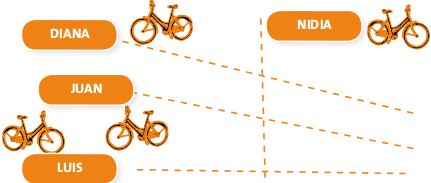
\includegraphics[scale=.55]{Images/Carreras_biciletas2.png}
\end{center}
\begin{center}
\begin{tabular}{|c|c|c|}
\hline 
\hspace*{20pt} Niños & Dibujos de los caminos & Descripción \\ 
\hline 
Juan y Diana &  &  \\ 
\hline 
Nidia y Luis &  &  \\ 
\hline 
Diana y Luis &  &  \\ 
\hline 
Diana y Nidia &  &  \\ 
\hline 
\end{tabular}
\end{center}
\section*{Evaluaci\'on}
\begin{itemize}
\item[2.] Dibuja dos pares de líneas paralelas y dos de líneas perpendiculares. Aprovecha las líneas de una cuadrícula.
\item[3.] Piensa en la siguiente afirmación y explica si es verdad o no: “todas líneas perpendiculares son secantes pero no todas las secantes son perpendiculares”.
\end{itemize}
 \section*{Lo que s\'e}
 Si realizaramos un mapa detallado de cada uno de los lugares por
los que nos movemos diarimente mientras realizamos nuestras
tareas diarias, el resultado sería un sin número de segmentos
unidos que podrían definir figuras y vértices.
\begin{itemize}
\item Lee la siguiente situación:
\end{itemize}
Guillermo quiere realizar un plano del recorrido que tiene
que hacer todos los días, para cumplir con sus tareas diarias.
\begin{enumerate}
\item[a.] Primera tarea: ordeñar las vacas y sacarlas a pastear.
\item[b.] Segunda tarea: recoger los huevos y darles de comer a las gallinas.
\item[c.] Tercera tarea: alimentar a los cerdos.
\item[d.] Cuarta tarea: llevar a las vacas de nuevo al corral.
\end{enumerate}
\begin{itemize}
\item Observa y copia la ubicación de los puntos que se muestran a
continuación. Piensa en el recorrido que hace Guillermo y traza
los caminos correspondientes.
\end{itemize}
\begin{center}
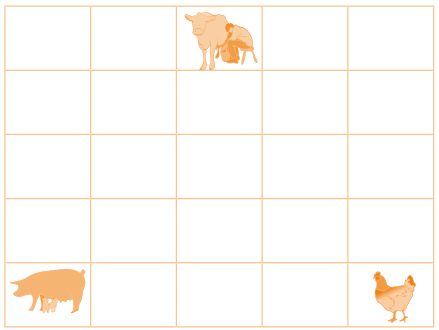
\includegraphics[scale=.55]{Images/animales_domesticos.png}
\end{center}
\begin{itemize}
\item ¿Qué figura se forma al trazar los recorridos?
\item Dibuja en tu cuaderno otra figura similar y explica
cuáles son las características comunes que tienen
entre sí.
\item Observa estas figuras y escribe en tu cuaderno qué las
diferencia de la que se obtuvo al dibujar el recorrido
hecho por Guillermo.
\begin{center}
\begin{tikzpicture}[scale=.75]
\filldraw[gray] (0,0)rectangle (3,2);
\filldraw[gray] (3.3,0)--(6.3,0)--(6.3,2) --cycle;
\filldraw[gray] (7.6,1) circle (1cm);
\end{tikzpicture}
\end{center}
\begin{itemize}
\item ¿Qué tipo de figura se formaría si antes de regresar las
vacas al corral, tuviera que ir a un sitio más? ¿Y a dos
sitios más? Realiza un dibujo que explique la situación
planteada.
\item Piensa en las actividades que realizas todos los días.
Recuerda la ubicación de los lugares en donde las haces
y representa los recorridos en un dibujo. ¿Qué figura
obtuviste?
\end{itemize}
\end{itemize}
\end{document}
